\documentclass[11pt,letterpaper]{article}
\usepackage[T1]{fontenc}
\usepackage[utf8]{inputenc}
\usepackage{lmodern}
\usepackage[margin=0.85in]{geometry}
\usepackage{microtype,amsmath,amssymb,booktabs,tabularx,graphicx,float}
\usepackage[font=small,labelfont=bf]{caption}
\usepackage[section]{placeins}
\usepackage{enumitem}
\usepackage[numbers,sort&compress]{natbib}
\usepackage{xurl}
\usepackage[hidelinks]{hyperref}
\hypersetup{pdftitle={Privacy-Fairness Tradeoffs in DP-SGD Employment Prediction},pdfauthor={Xiyin Xu and Shannon Saad}}
\setlist[itemize]{leftmargin=*,itemsep=2pt,topsep=4pt}
\setlength{\parskip}{4pt}
\setlength{\parindent}{0pt}
\setlength{\textfloatsep}{12pt}
\setlength{\floatsep}{10pt}
\graphicspath{{figures/}}
\newcommand{\eps}{\varepsilon}
\newcommand{\NA}{\textemdash}
\newcommand{\code}[1]{\texttt{\detokenize{#1}}}
\title{\vspace{-1.6em}Progress Report:\\Privacy--Fairness Tradeoffs in\\DP-SGD Employment Prediction\vspace{-0.4em}}
\author{Xiyin Xu \qquad Shannon Saad}
\date{November 18, 2026}

\begin{document}
\maketitle
\vspace{-1em}
\begin{center}\small\textit{Preliminary, single-run development-set results. Final test records have not been loaded.}\end{center}

\section{Motivation}
Differentially private stochastic gradient descent (DP-SGD) bounds the influence of individual training records through per-person gradient clipping and noise addition. Bagdasaryan et al.~\cite{bagdasaryan2019} showed that private training can reduce accuracy more for underrepresented groups. They examined accuracy parity and left other fairness notions to future work.

We extend this question to tabular employment prediction. We ask: (1) Does DP-SGD change accuracy disproportionately across sex and race groups? (2) Can Learning Fair Representations (LFR) and equalized-odds (EO) post-processing mitigate these disparities, and at what accuracy cost? (3) How do these effects vary with the privacy budget? Beyond accuracy parity, we assess independence, separation, and binary sufficiency. This is an experimental extension rather than a reproduction of the original datasets or architectures. No consistent effect would also be a valid finding.

\section{Task and data}
\textbf{Data and population.} We use California 2018 ACS 1-Year person records accessed through Folktables~\cite{ding2021}. The filtered employment task retains ages 17--89 (\code{AGEP > 16}, \code{AGEP < 90}) and person weights \code{PWGTP >= 1}.

\textbf{Target.} Following Folktables, $Y=1$ exactly when \code{ESR = 1}: civilian employed, at work~\cite{census2018}. Thus $Y=0$ includes unemployed people, people outside the labor force, employed civilians temporarily away from work (ESR 2), and Armed Forces categories (ESR 4--5). It does not mean ``unemployed.'' The positive-label rate is approximately 57\%.

\textbf{Inputs.} Fourteen source variables become 77 encoded columns: standardized age and one-hot categorical indicators. Recorded sex (\code{SEX}) and race (\code{RAC1P}) are audit metadata rather than direct inputs; correlated features can still carry group information. We dropped \code{ESP} (parents' employment status) on November 16 because 98.58\% of eligible records have missing values and its applicability is restricted, retaining every eligible person. Learned preprocessing is fitted only on reference data. GCL missingness is retained as an explicit category.

\begin{table}[H]
\centering\small
\begin{tabular}{lr}\toprule
Preparation stage & People\\\midrule
Raw records & 378,817\\
Excluded by age or weight rules & 76,177\\
Eligible records & 302,640\\\bottomrule
\end{tabular}
\caption{Population after eligibility filtering.}\label{tab:population}
\end{table}

\begin{table}[H]
\centering\small
\begin{tabularx}{\linewidth}{lrX}\toprule
Partition & People & Purpose\\\midrule
Reference & 30,264 & Fit preprocessing; later LFR (assumed public)\\
Training & 151,320 & Fit ordinary/private MLP; protected partition for DP training\\
Development & 30,264 & Evaluate pilots (assumed public)\\
Calibration & 30,264 & Learn EO decision rules later (assumed public)\\
Test & 60,528 & Final evaluation; untouched\\\bottomrule
\end{tabularx}
\caption{Fixed, disjoint data partitions.}\label{tab:splits}
\end{table}
Splits use person-level random assignment with seed 285, without stratification. Household-level separation has not been enforced and remains a protocol decision to review.

\section{Model, training, and privacy}
The MLP has architecture $77\rightarrow64\rightarrow32\rightarrow1$, ReLU hidden activations, and sigmoid output probabilities. We use binary cross-entropy, SGD with learning rate 0.05 and no momentum, nominal batch size 512, 20 epochs, threshold 0.5, and the final epoch without checkpoint selection. Ordinary and private runs share the architecture, initialization seed 285, data fingerprint, and these hyperparameters.

DP-SGD uses Opacus 1.6.0~\cite{opacus} with Poisson sampling, $q=1/296\approx0.00338$, full-model per-person clipping norm $C=1$, and R\'enyi-DP accounting. An epoch means 296 sampling steps, not exactly one visit to each person. Each run has 5,920 updates and
\[
\delta=\frac{1}{10n_{\mathrm{train}}}
       =\frac{1}{1{,}513{,}200}\approx6.61\times10^{-7}.
\]
\begin{table}[H]
\centering\small
\begin{tabular}{rrrr}\toprule
Target $\eps$ & Achieved $\eps$ & Noise multiplier & Runtime (s)\\\midrule
1 & 0.999 & 1.411 & 48\\
4 & 3.999 & 0.741 & 79\\
8 & 8.000 & 0.597 & 68\\\bottomrule
\end{tabular}
\caption{Per-run privacy accounting and measured CPU runtime.}\label{tab:privacy}
\end{table}

\textbf{Privacy scope.} Accountant bounds apply to training-partition records, conditional on fixed public reference, development, and calibration data and preprocessing fitted on the reference partition. Each $\eps$ describes one run. Basic composition for releasing all three private models gives a conservative bound of approximately $\eps=13.0$, $\delta=1.98\times10^{-6}$~\cite{dwork2014}. The ordinary baseline is not a private release, so the repository as a whole should not be described as DP. Pilots use research pseudorandom generators (\code{secure_mode = False}); sampling and noise seeds are not exported. Raw training-loss statistics are not released.

\section{Metrics}
For every group $g$, we compute accuracy, selection rate, true-positive rate (TPR), false-positive rate (FPR), positive predictive value (PPV), and negative predictive value (NPV). Define $\operatorname{gap}(r)=\max_g r_g-\min_g r_g$ for a rate $r$.

\begin{table}[H]
\centering\small
\begin{tabular}{ll}\toprule
Criterion & Reported gap\\\midrule
Accuracy parity & $\operatorname{gap}(\mathrm{accuracy})$\\
Independence & $\operatorname{gap}(\mathrm{selection\ rate})$\\
Separation (equalized odds) & $\max\{\operatorname{gap}(\mathrm{TPR}),\operatorname{gap}(\mathrm{FPR})\}$\\
Binary sufficiency & $\max\{\operatorname{gap}(\mathrm{PPV}),\operatorname{gap}(\mathrm{NPV})\}$\\\bottomrule
\end{tabular}
\caption{Statistical disparity criteria for binary decisions~\cite{fairmlbook,hardt2016}.}\label{tab:metrics}
\end{table}
Group-specific accuracy loss is
\[
L_g(\eps)=\mathrm{Acc}_{\mathrm{SGD},g}-\mathrm{Acc}_{\mathrm{DP},g}(\eps),
\]
evaluated on identical development records. Positive loss means lower accuracy under DP. We flag conditional denominators below 30 as unstable. If a required group rate is undefined, the full-group gap remains undefined; no category is silently excluded. These are predictive-disparity measurements on observational data, without causal identification of employment differences.

\section{Preliminary results}
\subsection{The baseline learns}
The non-private MLP reaches 77.08\% development accuracy (75.73\% balanced accuracy), compared with 57.01\% for majority-class prediction. Training loss decreases from 0.670 to 0.495 and development loss from 0.636 to 0.492. These trajectories show learning in this pilot; they do not establish generalization across seeds or the absence of overfitting beyond the observed run.

\subsection{Overall cost of private training}
\begin{table}[H]
\centering\small
\begin{tabular}{lrrrr}\toprule
Method & Target $\eps$ & Accuracy (\%) & Balanced (\%) & Loss (pp)\\\midrule
SGD & \NA & 77.08 & 75.73 & 0.00\\
DP-SGD & 1 & 75.82 & 73.67 & 1.26\\
DP-SGD & 4 & 75.81 & 73.69 & 1.27\\
DP-SGD & 8 & 75.78 & 73.63 & 1.30\\\bottomrule
\end{tabular}
\caption{Single-run development results. Achieved budgets appear in Table~\ref{tab:privacy}; pp denotes percentage points.}\label{tab:overall}
\end{table}
Private training costs approximately 1.3 percentage points of accuracy and 2.1 points of balanced accuracy (Figure~\ref{fig:accuracy}). Accuracy differs by only 0.04 points across the three private runs. We do not infer an $\eps$ trend from this spread: independent training repetitions and paired uncertainty estimates on the shared evaluation records are needed.

Balanced accuracy decreases more than accuracy as the private models predict the positive class more often. Overall selection rises from 63.2\% to approximately 68.5\%, TPR from 85.3\% to approximately 88.9\%, and FPR from 33.9\% to approximately 41.5\%.
\begin{figure}[H]
\centering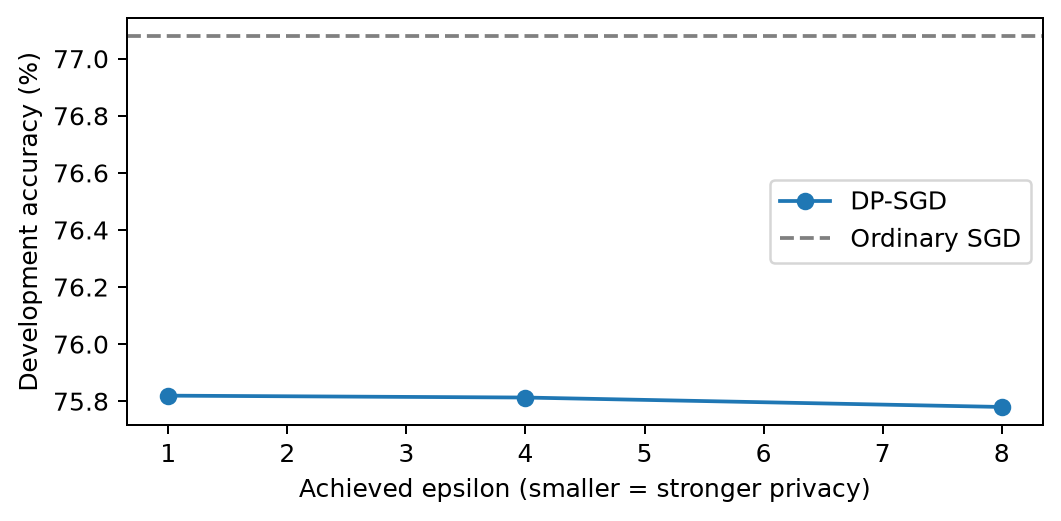
\includegraphics[width=0.76\linewidth]{accuracy_vs_epsilon.png}
\caption{Development accuracy versus achieved privacy budget. The dashed line is ordinary SGD. Each private point is one run; no uncertainty interval has yet been estimated.}\label{fig:accuracy}
\end{figure}

\subsection{Accuracy loss by group}
\begin{table}[H]
\centering\small\setlength{\tabcolsep}{4pt}
\begin{tabular}{lrrrrr}\toprule
Group & $n$ & SGD (\%) & $L_g(1)$ & $L_g(4)$ & $L_g(8)$\\\midrule
Male & 14,826 & 80.48 & 0.90 & 0.93 & 0.91\\
Female & 15,438 & 73.81 & 1.61 & 1.59 & 1.67\\
White alone & 18,889 & 77.33 & 1.24 & 1.18 & 1.23\\
Black alone & 1,500 & 79.73 & 1.07 & 1.27 & 1.40\\
Asian alone & 5,017 & 76.78 & 1.63 & 1.69 & 1.65\\
Some other race alone & 3,299 & 75.02 & 0.67 & 0.97 & 0.88\\
Two or more races & 1,179 & 77.27 & 1.70 & 1.61 & 1.78\\\bottomrule
\end{tabular}
\caption{Group accuracy losses in percentage points, indexed by target $\eps$. Race rows show groups with at least 500 development records; sex rows include both recorded categories.}\label{tab:groups}
\end{table}
The female group loses approximately 1.6--1.7 points versus 0.9 points for the male group at each budget. This is consistent with disproportionate loss in the lower-accuracy sex group, but remains suggestive with one run per budget. Larger race groups lose approximately 0.7--1.8 points, with no consistent ordering across budgets (Figure~\ref{fig:groups}).

Smaller race groups are retained in full audit tables but omitted from Table~\ref{tab:groups} and the plot: American Indian alone ($n=202$), other American Indian/Alaska Native category ($n=81$), Native Hawaiian/Other Pacific Islander alone ($n=95$), and Alaska Native alone ($n=2$). For example, a 3.16-point loss in the Pacific Islander group corresponds to only three records.
\begin{figure}[H]
\centering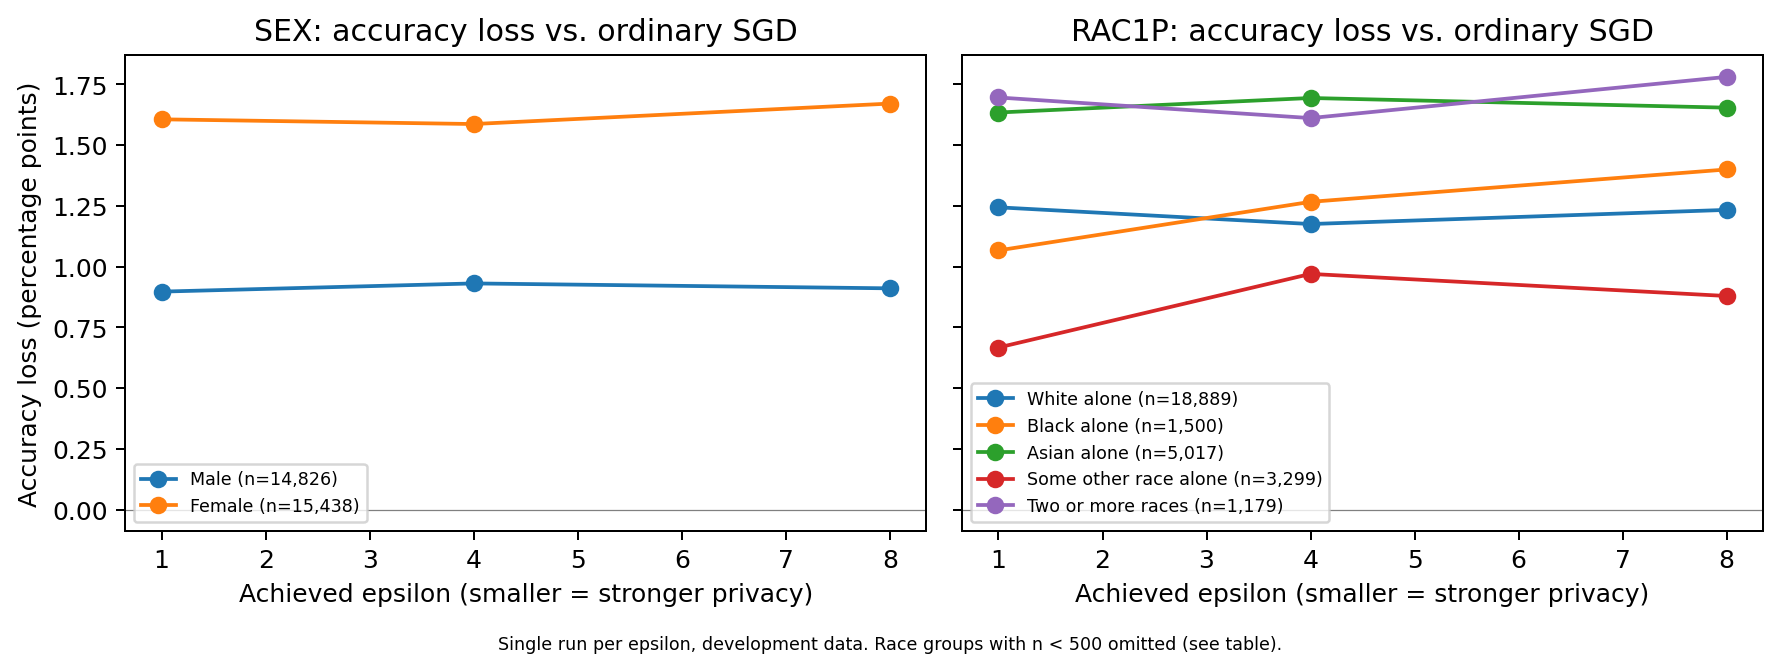
\includegraphics[width=\linewidth]{group_loss_vs_epsilon.png}
\caption{Accuracy loss relative to ordinary SGD by sex and larger race groups. The race plot uses a display threshold of $n\ge500$, separate from the conditional-denominator flag of 30 used for rate stability.}\label{fig:groups}
\end{figure}

\subsection{Fairness gaps}
\begin{table}[H]
\centering\small
\begin{tabular}{lrrrr}\toprule
Method & Accuracy & Independence & Separation & Sufficiency\\\midrule
SGD & 6.67 & 0.64 & 12.01 & 12.58\\
DP-SGD, $\eps\approx1$ & 7.38 & 0.78 & 11.38 & 12.12\\
DP-SGD, $\eps\approx4$ & 7.33 & 0.91 & 11.51 & 12.16\\
DP-SGD, $\eps\approx8$ & 7.43 & 0.87 & 11.54 & 12.19\\\bottomrule
\end{tabular}
\caption{Sex-group disparity gaps in percentage points. Lower means closer agreement with that particular criterion.}\label{tab:sexgaps}
\end{table}
The sex accuracy gap widens by approximately 0.7 points, while separation and sufficiency gaps shrink by approximately 0.5 points. Different criteria move in different directions; run-to-run variability has not yet been measured. The baseline separation gap is driven mainly by FPR (27.1\% for males versus 39.1\% for females); its TPR gap is approximately 0.2 points. Selection rates are nearly equal (63.0\% versus 63.5\%), despite different label base rates (61.5\% versus 52.6\%). Thus small independence gaps coexist with accuracy and FPR differences.

For race, the accuracy gap is 31.2 points under SGD and approximately 32.2 under DP; independence rises from 69.5 to approximately 77 points. These extremes are dominated by tiny groups, including Alaska Native alone ($n=2$, with no positive labels). Full-race separation and sufficiency are undefined because required conditional denominators are absent. They are not reported as zero, and groups are not excluded to manufacture a defined full-population gap (Figure~\ref{fig:fairness}). We plan a separately labeled, prespecified White-alone/Black-alone comparison, alongside the full audit.
\begin{figure}[H]
\centering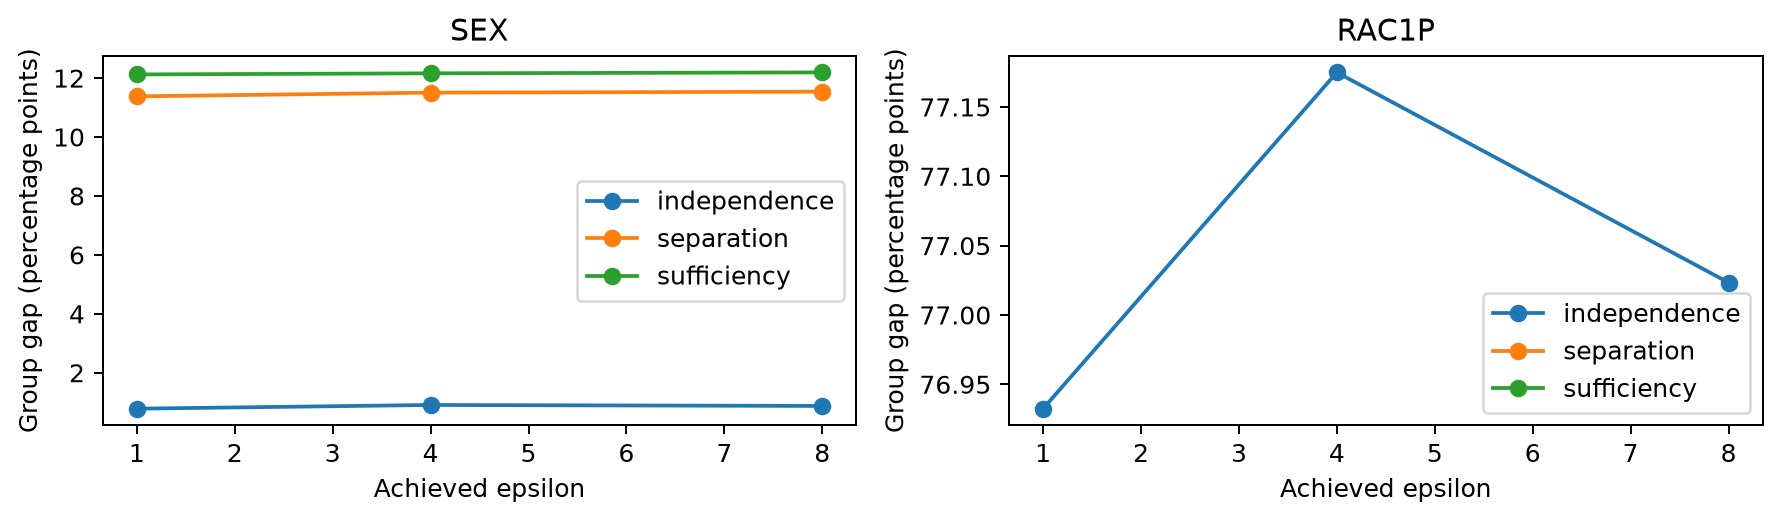
\includegraphics[width=\linewidth]{fairness_gaps.png}
\caption{Disparity gaps across private pilots. Full-race separation and sufficiency have no plotted values because they are undefined. Their legend entries do not imply zero gaps.}\label{fig:fairness}
\end{figure}

\section{Limitations}
\begin{itemize}
\item \textbf{Single initialization and one run per budget.} Independent sampling/noise variation cannot yet be separated from systematic budget effects.
\item \textbf{Mechanism confounding.} Ordinary SGD uses shuffled fixed batches; DP-SGD combines Poisson sampling, clipping, and noise. Losses cannot be attributed to noise alone. A sampling-matched or clipping-only diagnostic is planned.
\item \textbf{Development-only evaluation.} Test outcomes remain unused. Development records are assumed public auxiliary data in the privacy design.
\item \textbf{Small groups.} Several race and intersectional groups have conditional denominators below 30. Some race-by-sex calibration cells are empty or single-label, preventing a full intersectional EO fit without revising the analysis population.
\item \textbf{Target definition.} ESR 1 excludes employed civilians temporarily away and military employment. A broader target remains a pending decision.
\item \textbf{Unweighted metrics.} Results describe the sample, rather than survey-weighted California population estimates.
\end{itemize}

\section{Remaining work}
We will compare LFR~\cite{zemel2013}, which targets statistical parity in a learned representation, with EO post-processing~\cite{hardt2016}. Each method will have non-private controls and matched cohorts.
\begin{table}[H]
\centering\small
\begin{tabularx}{\linewidth}{lX}\toprule
Dates & Planned work\\\midrule
Nov.\ 19--21 & EO for sex/race with non-private controls; audit both attributes for every output.\\
Nov.\ 22--24 & LFR on reference data: sex first, then a supported binary-race cohort; matched ordinary/private MLPs.\\
Nov.\ 25 & Freeze cohorts, splits, preprocessing, tuning rules, seeds, and metrics.\\
Nov.\ 25--30 & Main grid: SGD, DP-SGD, LFR+SGD, LFR+DP-SGD, SGD+EO, and DP-SGD+EO; $\eps\in\{0.5,1,2,4,8\}$ (fallback $\{1,4,8\}$); at least three training seeds.\\
Dec.\ 1--3 & Final test evaluation, uncertainty intervals, and figures.\\
Dec.\ 4--7 & Final report; submission by December 7.\\\bottomrule
\end{tabularx}
\caption{Schedule for completing the experiments and final report.}\label{tab:timeline}
\end{table}

\section{Reproducibility}
Settings are recorded in \path{configs/baseline.json} and \path{configs/dp_pilot.json}. Entry points are \path{scripts/prepare_data.py}, \path{scripts/train_baseline.py}, \path{scripts/train_dp.py}, \path{scripts/report_dp.py}, and \path{scripts/plot_group_losses.py}. Metric and private-training checks run with \code{python -m unittest discover -s tests}.

Completed DP runs refuse to be overwritten. A replicate requires a copied configuration with a new output directory; additional released runs compose privacy cost. Raw data, checkpoints, and row-level predictions are excluded from Git. Aggregate tables and plots are derived from saved development results without retraining or loading test records.

\begingroup\small
\bibliographystyle{plainnat}
\bibliography{references}
\endgroup
\end{document}
